% Document settings
\documentclass[11pt]{article}
\usepackage[margin=1in]{geometry}
\usepackage{graphicx}
\usepackage{multirow}
\usepackage{setspace}
\usepackage{amsmath,amssymb,gensymb,epsfig, epstopdf}
\usepackage{xcolor}
\pagestyle{plain}
\setlength\parindent{0pt}
\setlength{\parskip}{1em}

\begin{document}

% Header
\textbf{Nitin Kapania} \\
\textbf{Modeling the Interaction Between a Pedestrian and Autonomous Vehicle at a Mid-Block Intersection} \\ 

\section{Problem Formulation}
Consider the problem of an autonomous vehicle attempting to drive past an unsignalized, ``mid-block" crosswalk, shown in Fig.~\ref{img:example}. A pedestrian is simultaneously walking towards the intersection, but has not entered. 

\begin{center}
   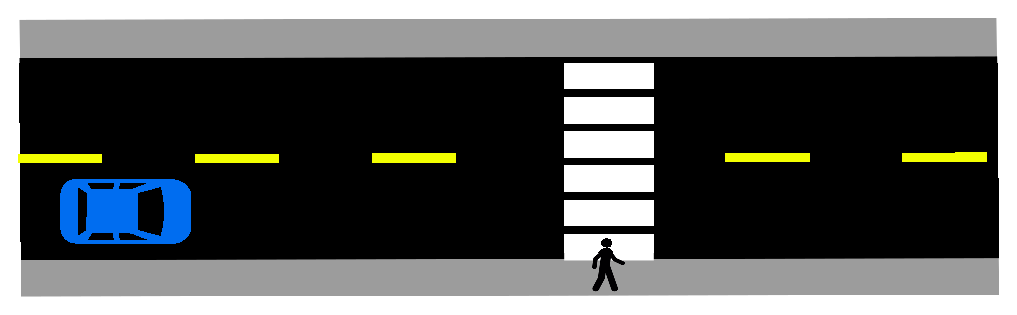
\includegraphics[width=.8\textwidth]{Images/example.eps}
   \label{img:example}
\end{center}

What should the autonomous vehicle do? Should the vehicle always stop as soon as a pedestrian is observed near a cross-walk? Can the AV make the decision to speed up and cross before the pedestrian is in the intersection? If so, how can it communicate intent to the pedestrian? Likewise, can it interpret signals from the pedestrian to understand whether the pedestrian is set on crossing? 

Uncontrolled mid-block intersections, like the one shown in Fig.~\ref{img:example}, pose the ambiguity of right of way. These laws are dictated on a state-by-state basis. While several states (e.g. Minnesota, Georgia, Maryland) have ``must-stop" rules for uncontrolled intersections, other states have ``must yield" rules. For example, vehicles in Arkansas must yield once a pedestrian is in any portion of the roadway, while vehicles in Alabama require motorists to yield to a pedestrian either on the same half of the road or approaching from the opposite side of the roadway. 

Given this ambiguity, there is a clear need to study the interaction between the pedestrian and the autonomous vehicle. Most human drivers and pedestrians do not know the explicit laws of their state, but safely navigate pedestrian interactions nonetheless. 

Several research questions can be posed for the following situation:

\begin{itemize}  
	\item Can we come up with a mathematical formulation describing this situation? 
	\item Can we superimpose this mathematical model with real-world data of pedestrian intersection crossings? 
	\item Can this formulation, combined with real-world data, be used to predict realistic 
	interaction scenarios?
	\item Can we design control policies for the vehicle that maintain a high standard of safety while also enabling robust traffic flow? 
\end{itemize}


\section{Prior Work}

There is a wide body of literature focused on understanding pedestrian behavior. In terms of microscopically modeling the dynamics of pedestrian motion, Batkovic et al. \cite{Batkovic} presented a mathematical model to predict pedestrian motion over a finite horizon based on a map of the road configuration, with a focus on low computational complexity for autonomous driving. Karasev et al. modeled pedestrian intent using a Markov Decision Process \cite{Karasev2016}. 

Another segment of the literature is focused on developing macroscopic predictive models for pedestrian crossing. These approaches typically study the parallel issues of pedestrian crossing behavior or driver yielding behavior based on experimental observation and date as early as 1975 \cite{Katz1975}. Schroeder and Rouphail \cite{Schroeder2011} explored factors associated with driver yielding behavior at unsignalized pedestrian crossings. Using logistic regression, the authors found that drivers are more likely to yield to assertive pedestrians who walk briskly in their approach to a crosswalk. Kadali and Perumal \cite{RaghuramKadali2012} studied the ``gap acceptance" behavior of pedestrians at mid-block crosswalks through a video graphic survey, and found that the gap accepted for crossing was explained by factors such as crossing direction, vehicle speed, and pedestrian age. Yannis et al. \cite{Yannis2013} and \cite{Sun2002} also found that gap acceptance was influenced by the size of the oncoming vehicle and the presence of other pedestrians.  Lee and Aty \cite{Lee2005} studied interactions in the form of crashes, and found crashes were linked with higher daily traffic. 

Another branch of literature specifically studies the interaction between pedestrians and autonomous vehicles at crosswalks. An excellent review of these studies was conducted by \cite{Rasouli}. As an example, Rothenbucher et al. \cite{Rothenbucher2016} studied the interaction between pedestrians and driverless vehicles by constructing a car seat costume to disguise a driver. The authors noted that pedestrians overall managed interactions at crosswalks effectively, but later mentioned increased uncertainty about the autonomous vehicles behavior. To improve the issue of trust, several researchers have developed external interfaces to more clearly broadcast the intent of the autonomous vehicle \cite{Matthews}, \cite{Lagstrom2015}. 

Several real-world studies of AV-pedestrian interaction noted that once a local population learned a vehicle was programmed to be perfectly safe, pedestrians would regularly take advantage of the AV and walk in front of it. \cite{Madigan}. This illustrates an issue with automated driving in that an overly conservative crossing algorithm will often be taken advantage of or cause confusion among pedestrians. Camara et al \cite{Camara2018} attempted to model the natural negotation for priority between a pedestrian and an AV at an intersection using the framework of ``sequential chicken" adopted from game theory. Chen et al. \cite{Chen} notes the need for a tradeoff between passive and aggressive driving behavior, and developed a stochastic model of pedestrian behavior to evaluate proposed AV control policies. Policies for pedestrian interaction are also developed by \cite{Bandyopadhyay}, who proposes a Mixed-observable Markov Decision Process (MOMDP) to incorporate the intention uncertainty of a pedestrian. A POMDP formulation is also proposed by Thornton \cite{Goldenstein2013}, who proposes navigation of the pedestrian uncertainty through value-sensitive design.    


\section{Proposed Research}

I have a couple of ideas to get into this field, but could use more inspiration

\begin{itemize}
	\item Collecting a dataset of ambiguous pedestrian-vehicle interaction exemplars from the VAIL simulator. 
	\subitem
		It is likely that we can use our simulator capabilities to set up an environment where two humans can negotiate a tricky mid-block intersection. The 
		initial settings can be set up so it is ambiguous whether the car should yield or go forward
	
	\subitem
		One human can be operating a vehicle, while another human can operate as a pedestrian in the world using a joystick.

	\item Showing the inherent uncertainty of the problem by simulating a pedestrian and vehicle acting independently at a mid-block intersection. Given a traffic law 
	for a certain state, we can show that given uncertainty, the traffic flow is inherently suboptimal.

	\subitem 
		However, given some communication of intent (either through a signaling device on the AV) or through assertive or intent-giving motion from the AV, we can optimize traffic flow while avoiding collision probability. 



\end{itemize} 



\bibliographystyle{plain}
\bibliography{Bibliography}

\end{document}

